\documentclass{article}
\usepackage[T1]{fontenc}
\usepackage{lmodern}
\usepackage{graphicx}
\usepackage{amsmath,amssymb}
\usepackage[a4paper,margin=2cm]{geometry}
\usepackage[absolute,overlay]{textpos}
\setlength{\TPHorizModule}{1mm}
\setlength{\TPVertModule}{1mm}
\usepackage[indonesian]{babel}
\usepackage{hyperref}
\setlength{\emergencystretch}{2em}
% unit: Halaman 19

\begin{document}

% === Halaman 19 (llm) ===

\begin{itemize}
    \item Contoh:
\end{itemize}

\[ P+P = 2P \]

\vspace{10mm}

\[ m = \frac{dy}{dx} = \frac{3x_p^2 + a}{2y_p} \]

Koordinat Titik R:
\[ x_r = m^2 - 2x_p \]
\[ y_r = m(x_p - x_r) - y_p \]

\vspace{40mm}

Sumber gambar: Debdeep Mukhopadhyay, Elliptic Curve Cryptography, Dept of Computer Sc and Engg IIT Madras

% deskripsi: Grafik kurva eliptik dengan persamaan y^2 = x^3 - 3x + 5 yang menunjukkan operasi penjumlahan titik P + P = 2P, lengkap dengan titik P, R, dan -R serta garis singgung.
% bbox normalisasi: [0.3900, 0.2200, 0.6700, 0.8200]
\begin{textblock*}{58.80mm}(81.90mm,65.34mm)
\noindent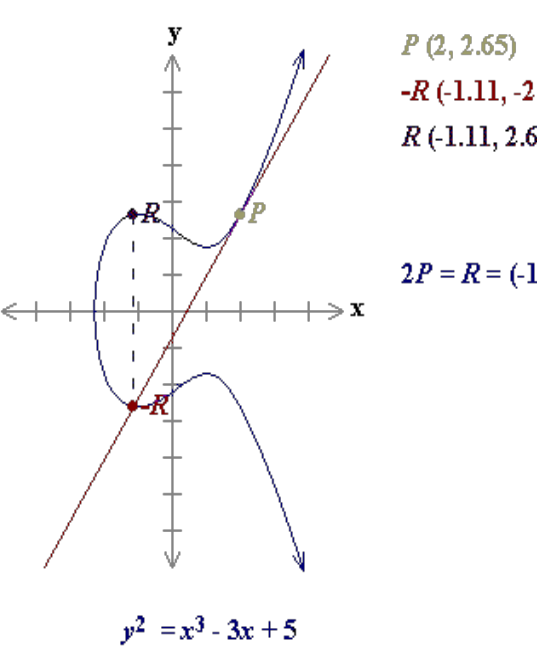
\includegraphics[width=58.80mm,height=178.20mm]{../../images/llm/page_019_img_01.png}%
\end{textblock*}

\end{document}
